\section{Results}
\subsection{Exploratory Data Analysis}

\subsubsection{Distribution of Securities by Type}

\begin{figure}[!htbp]
    \centering
    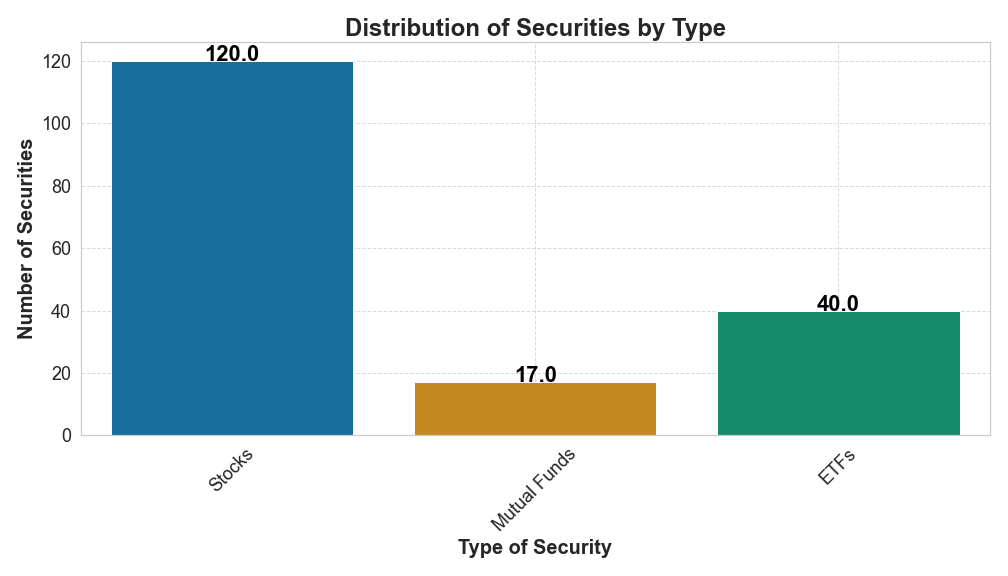
\includegraphics[width=0.8\textwidth]{../Figures/histogram_security_count.png}
    \caption{Distribution of Securities by Type}
    \label{fig:distribution_of_securities}
\end{figure}

\subsubsection{Cumulative Returns by Security Type}

\begin{figure}[!htbp]
    \centering
    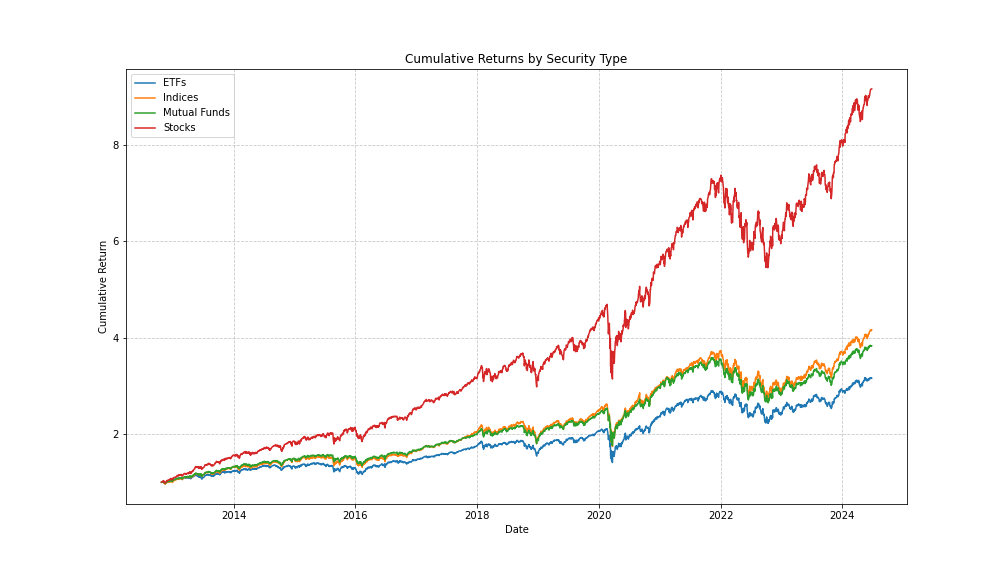
\includegraphics[width=0.8\textwidth]{../Figures/cumulative_returns_by_type.png}
    \caption{Cumulative Returns Over Time by Security Type}
    \label{fig:cumulative_returns_by_type}
    \subcaption The majority of the securities analyzed are stocks, followed by ETFs and mutual funds. Stocks exhibit the highest cumulative return over time, indicating a higher potential for long-term growth compared to ETFs and mutual funds.
\end{figure}

\newpage

\subsection{Optimal Portfolios}


\begin{figure}[!htbp]
    \centering
    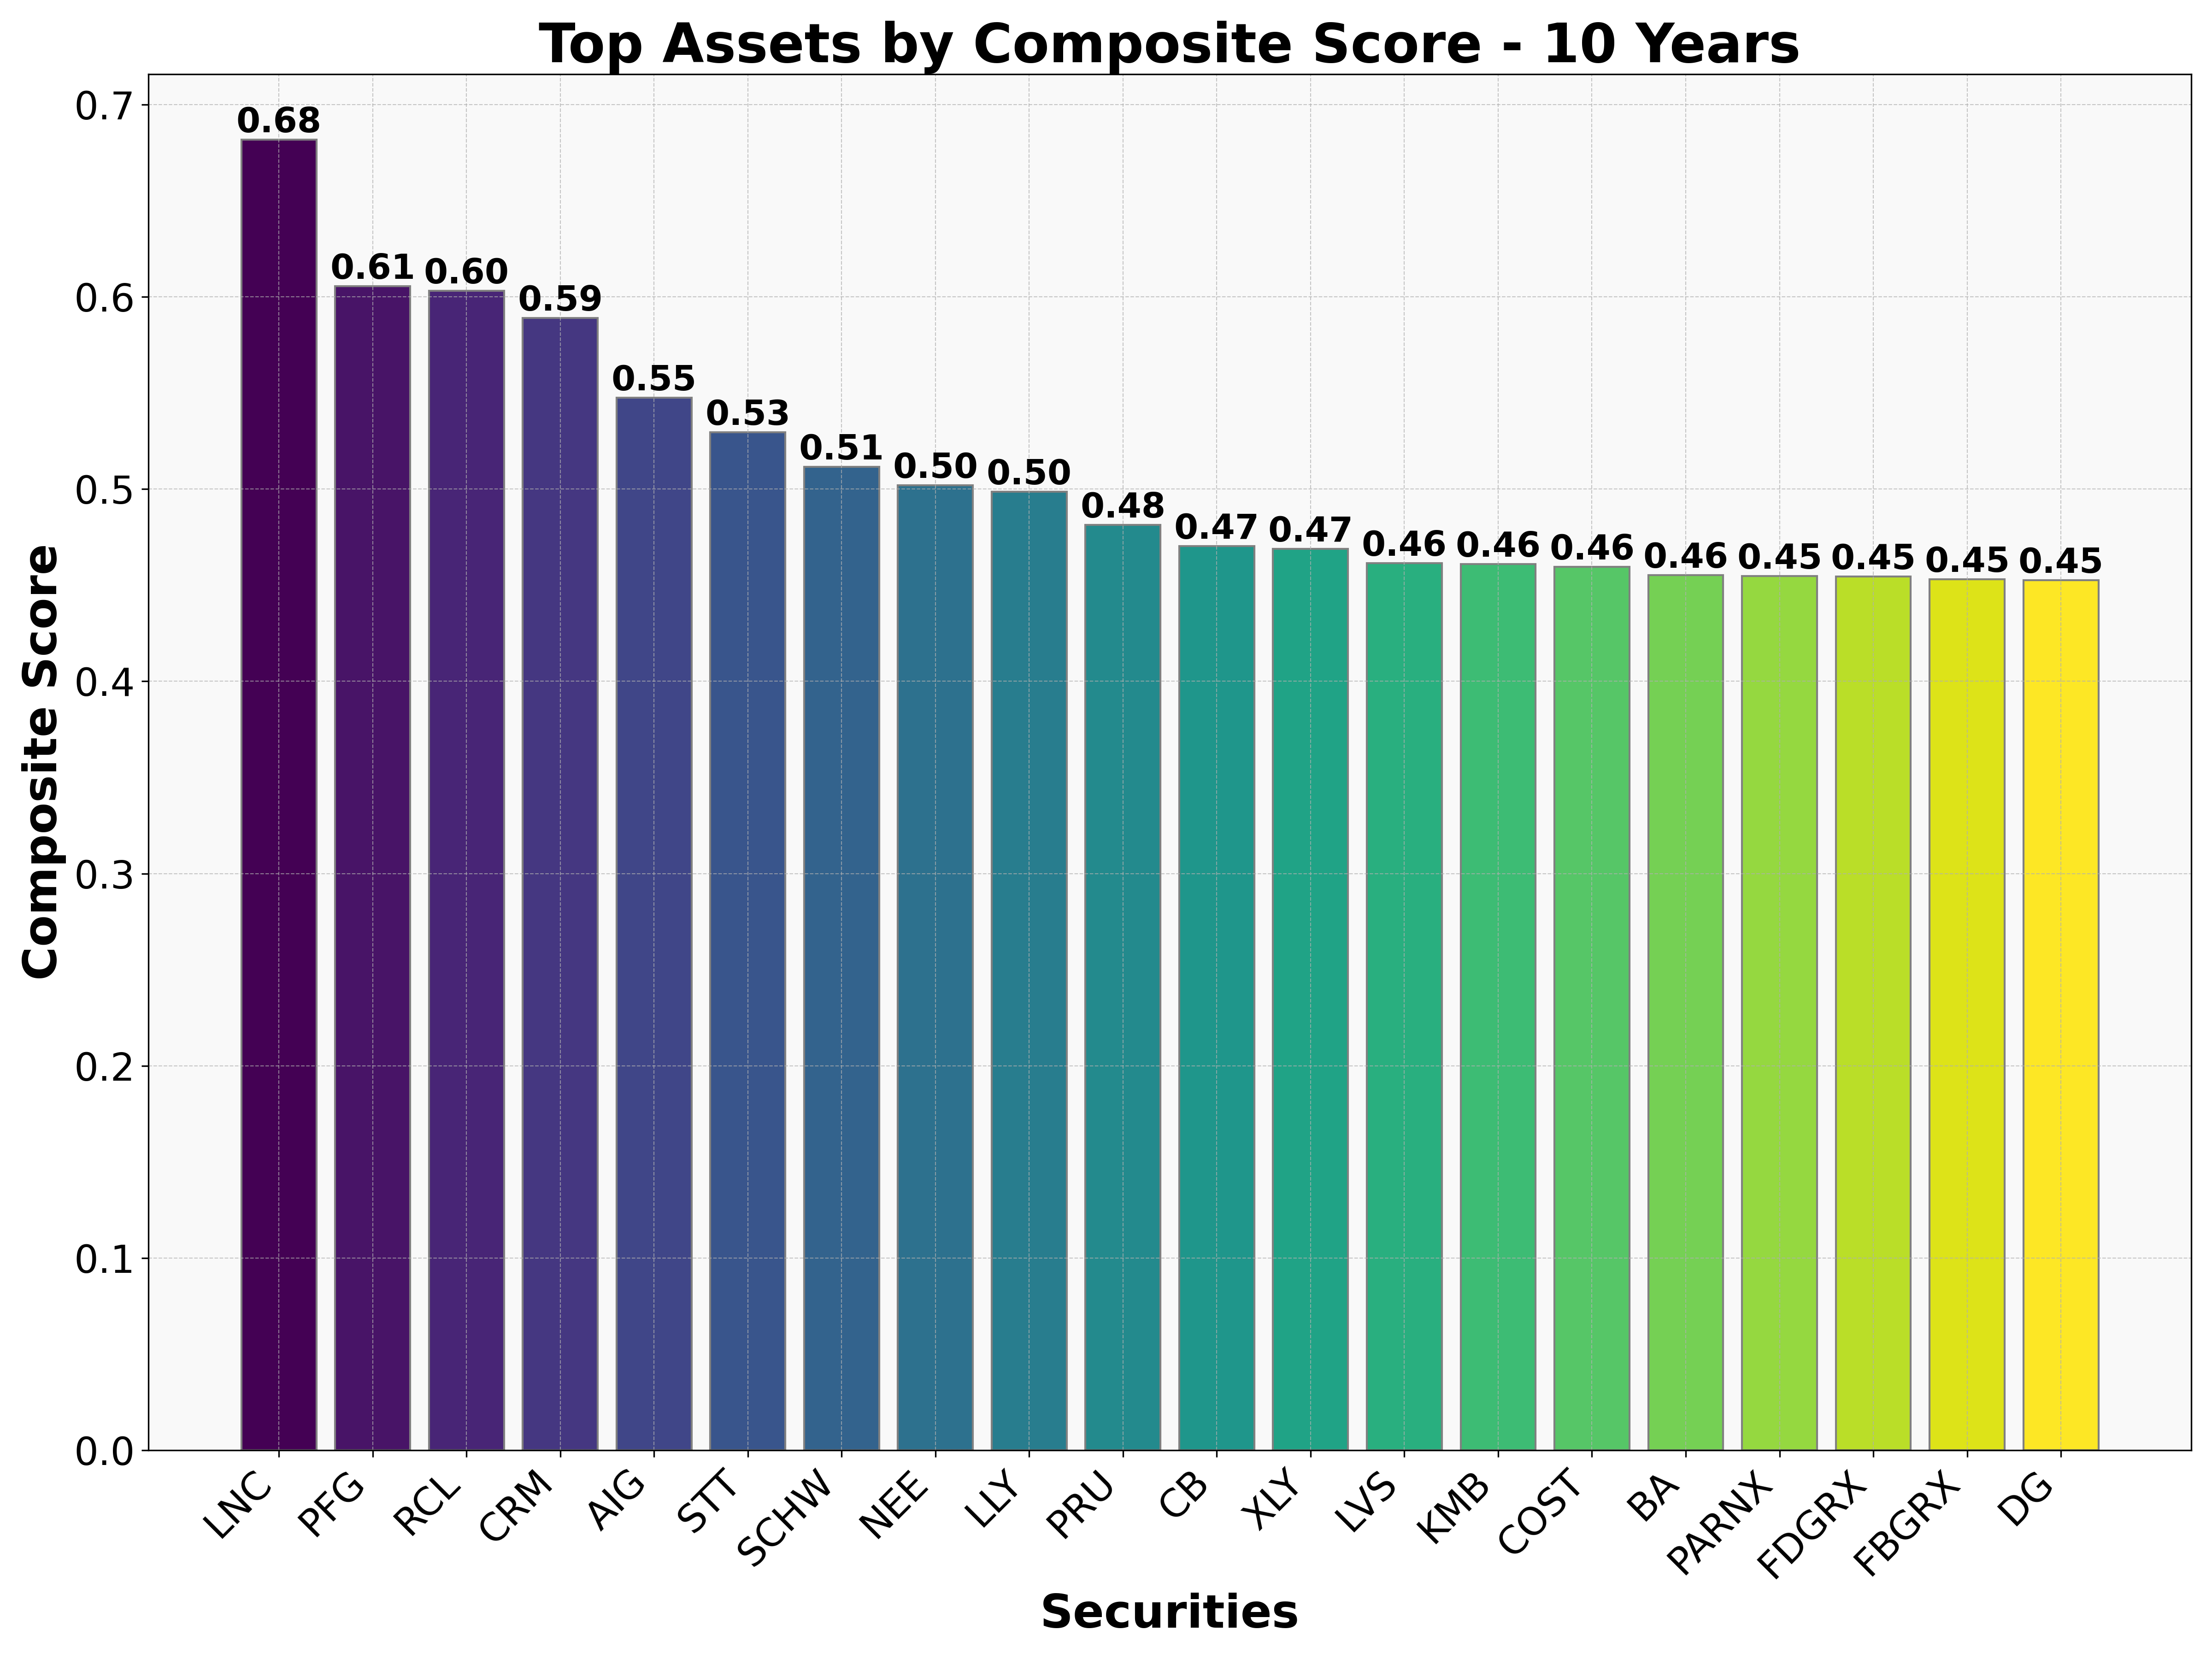
\includegraphics[width=0.8\textwidth]{../Figures/top_assets_composite_score_10_years.png}
    \caption{Top Assets by Composite Score (10 Years)}
    \label{fig:top_assets_10y}
\end{figure}

\begin{figure}[!htbp]
    \centering
    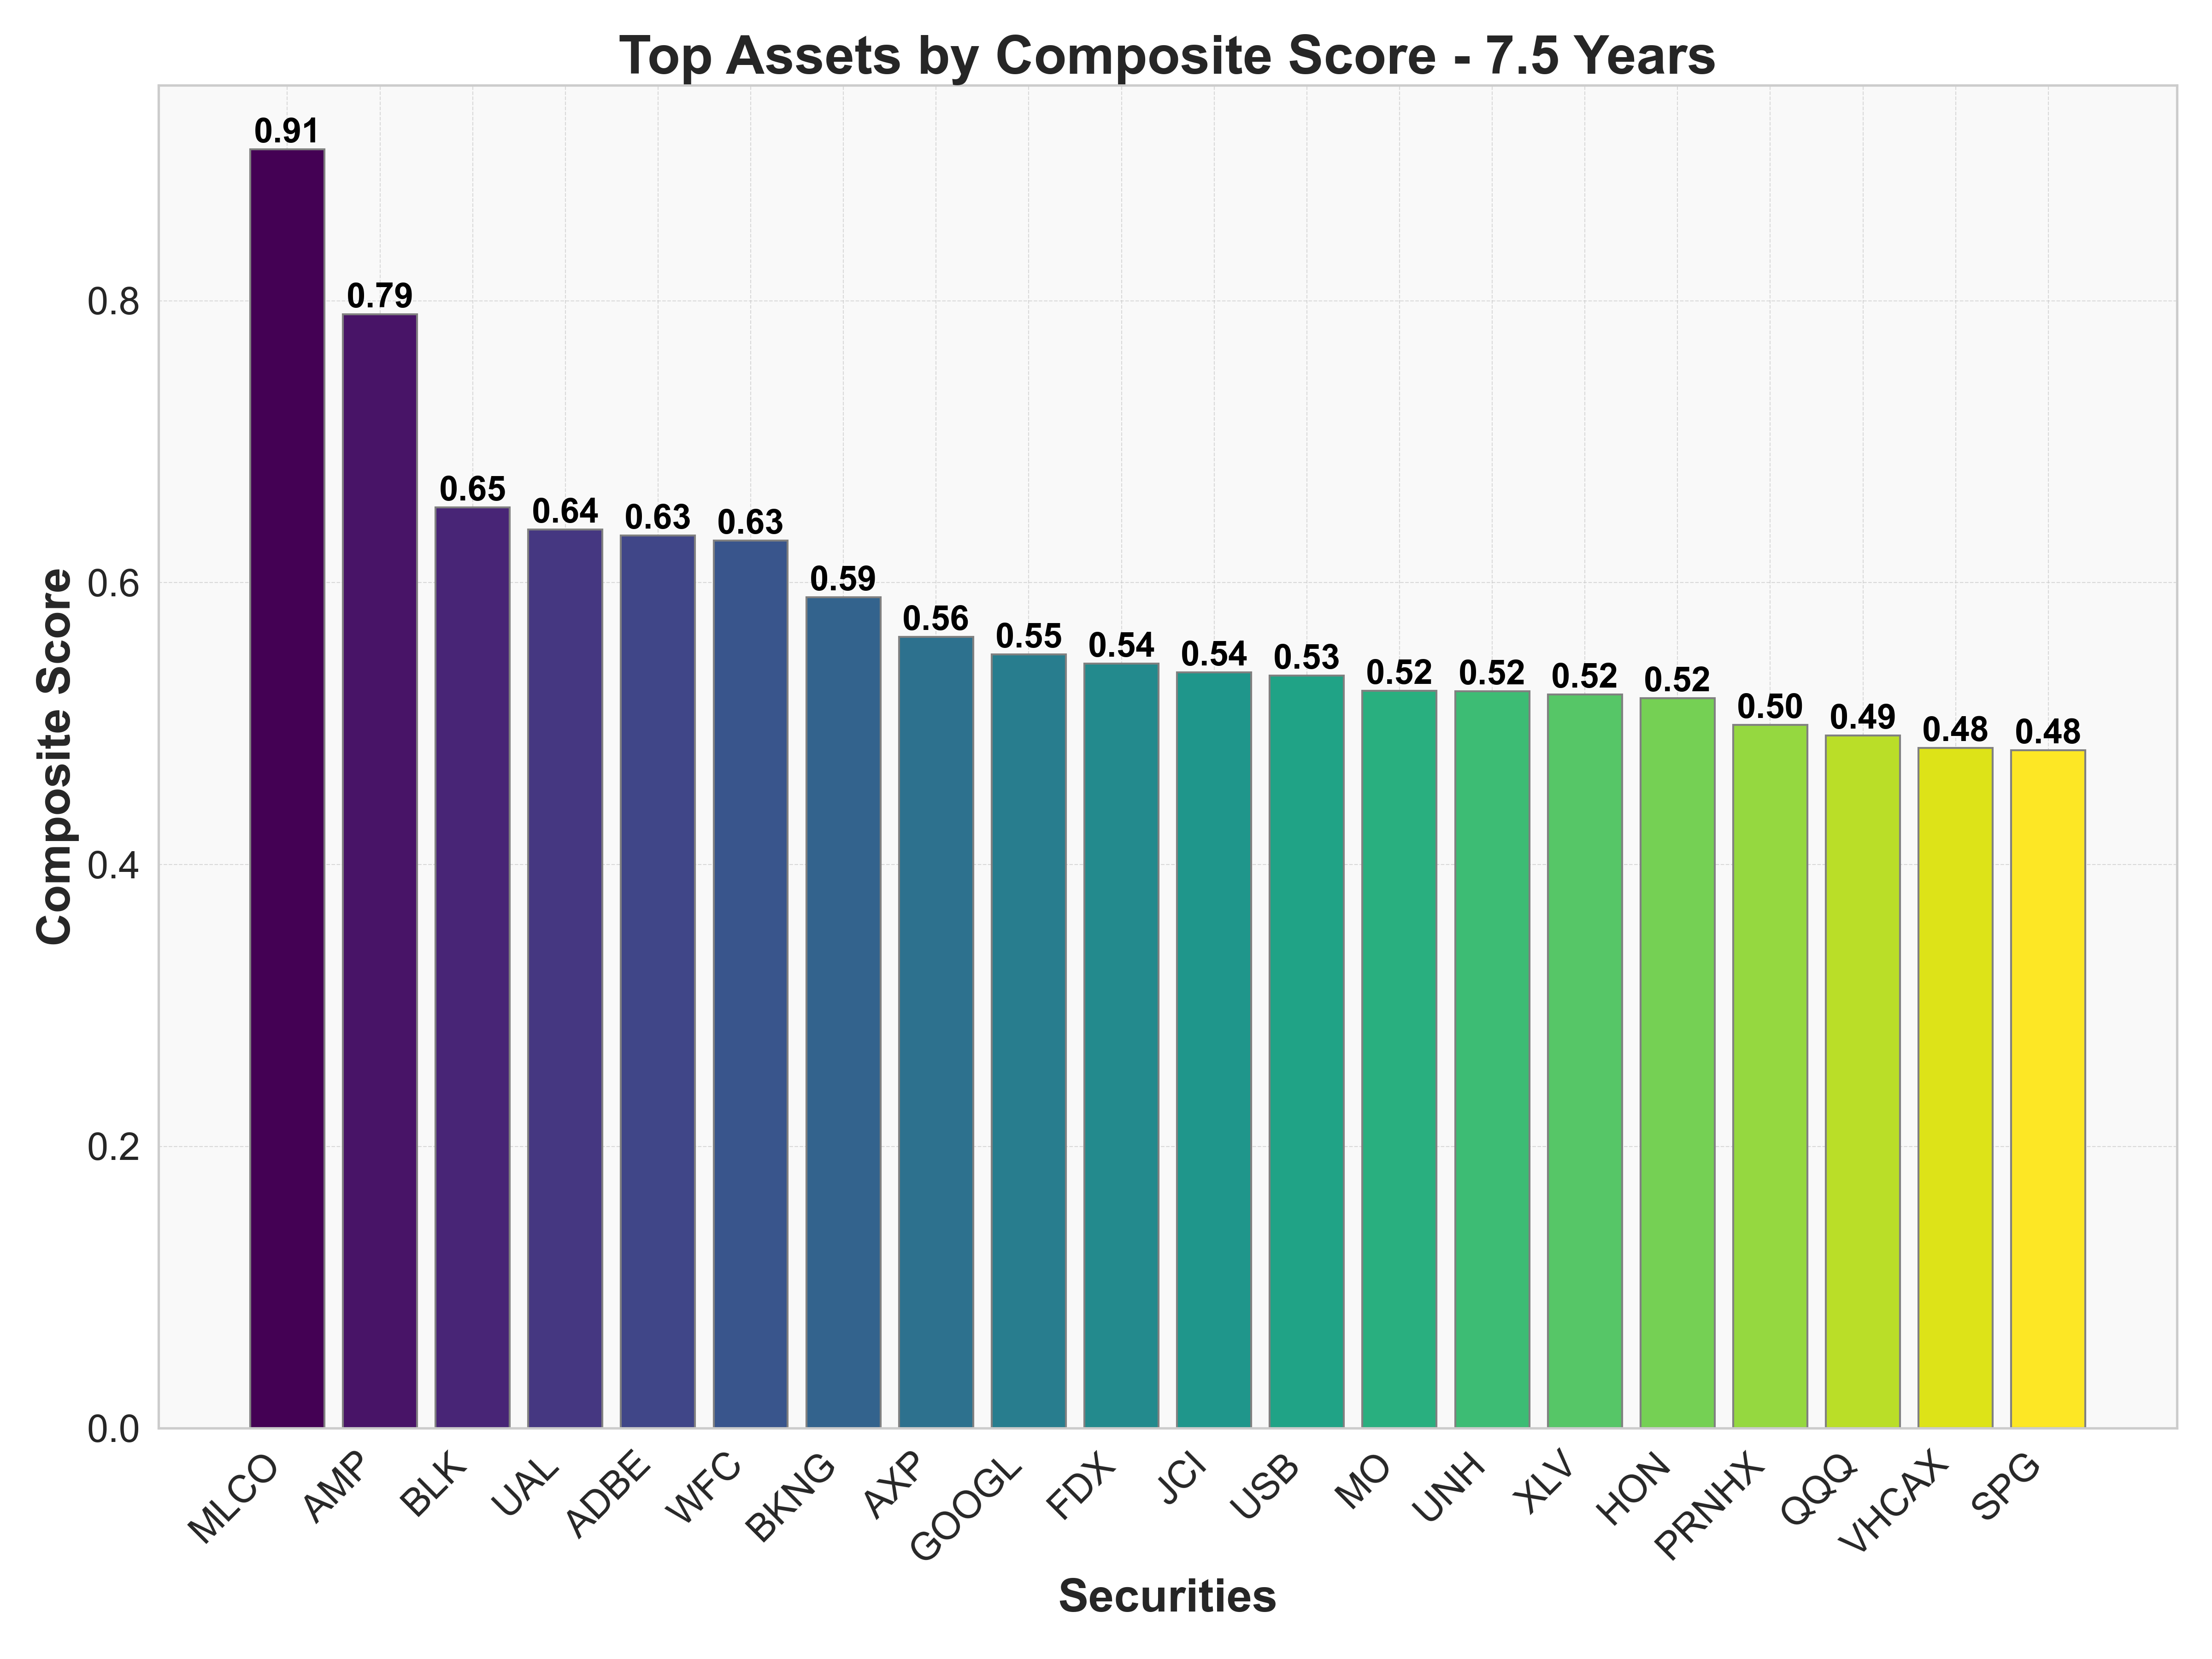
\includegraphics[width=0.8\textwidth]{../Figures/top_assets_composite_score_7_5_years.png}
    \caption{Top Assets by Composite Score (7.5 Years)}
    \label{fig:top_assets_7_5y}
\end{figure}

\begin{figure}[!htbp]
    \centering
    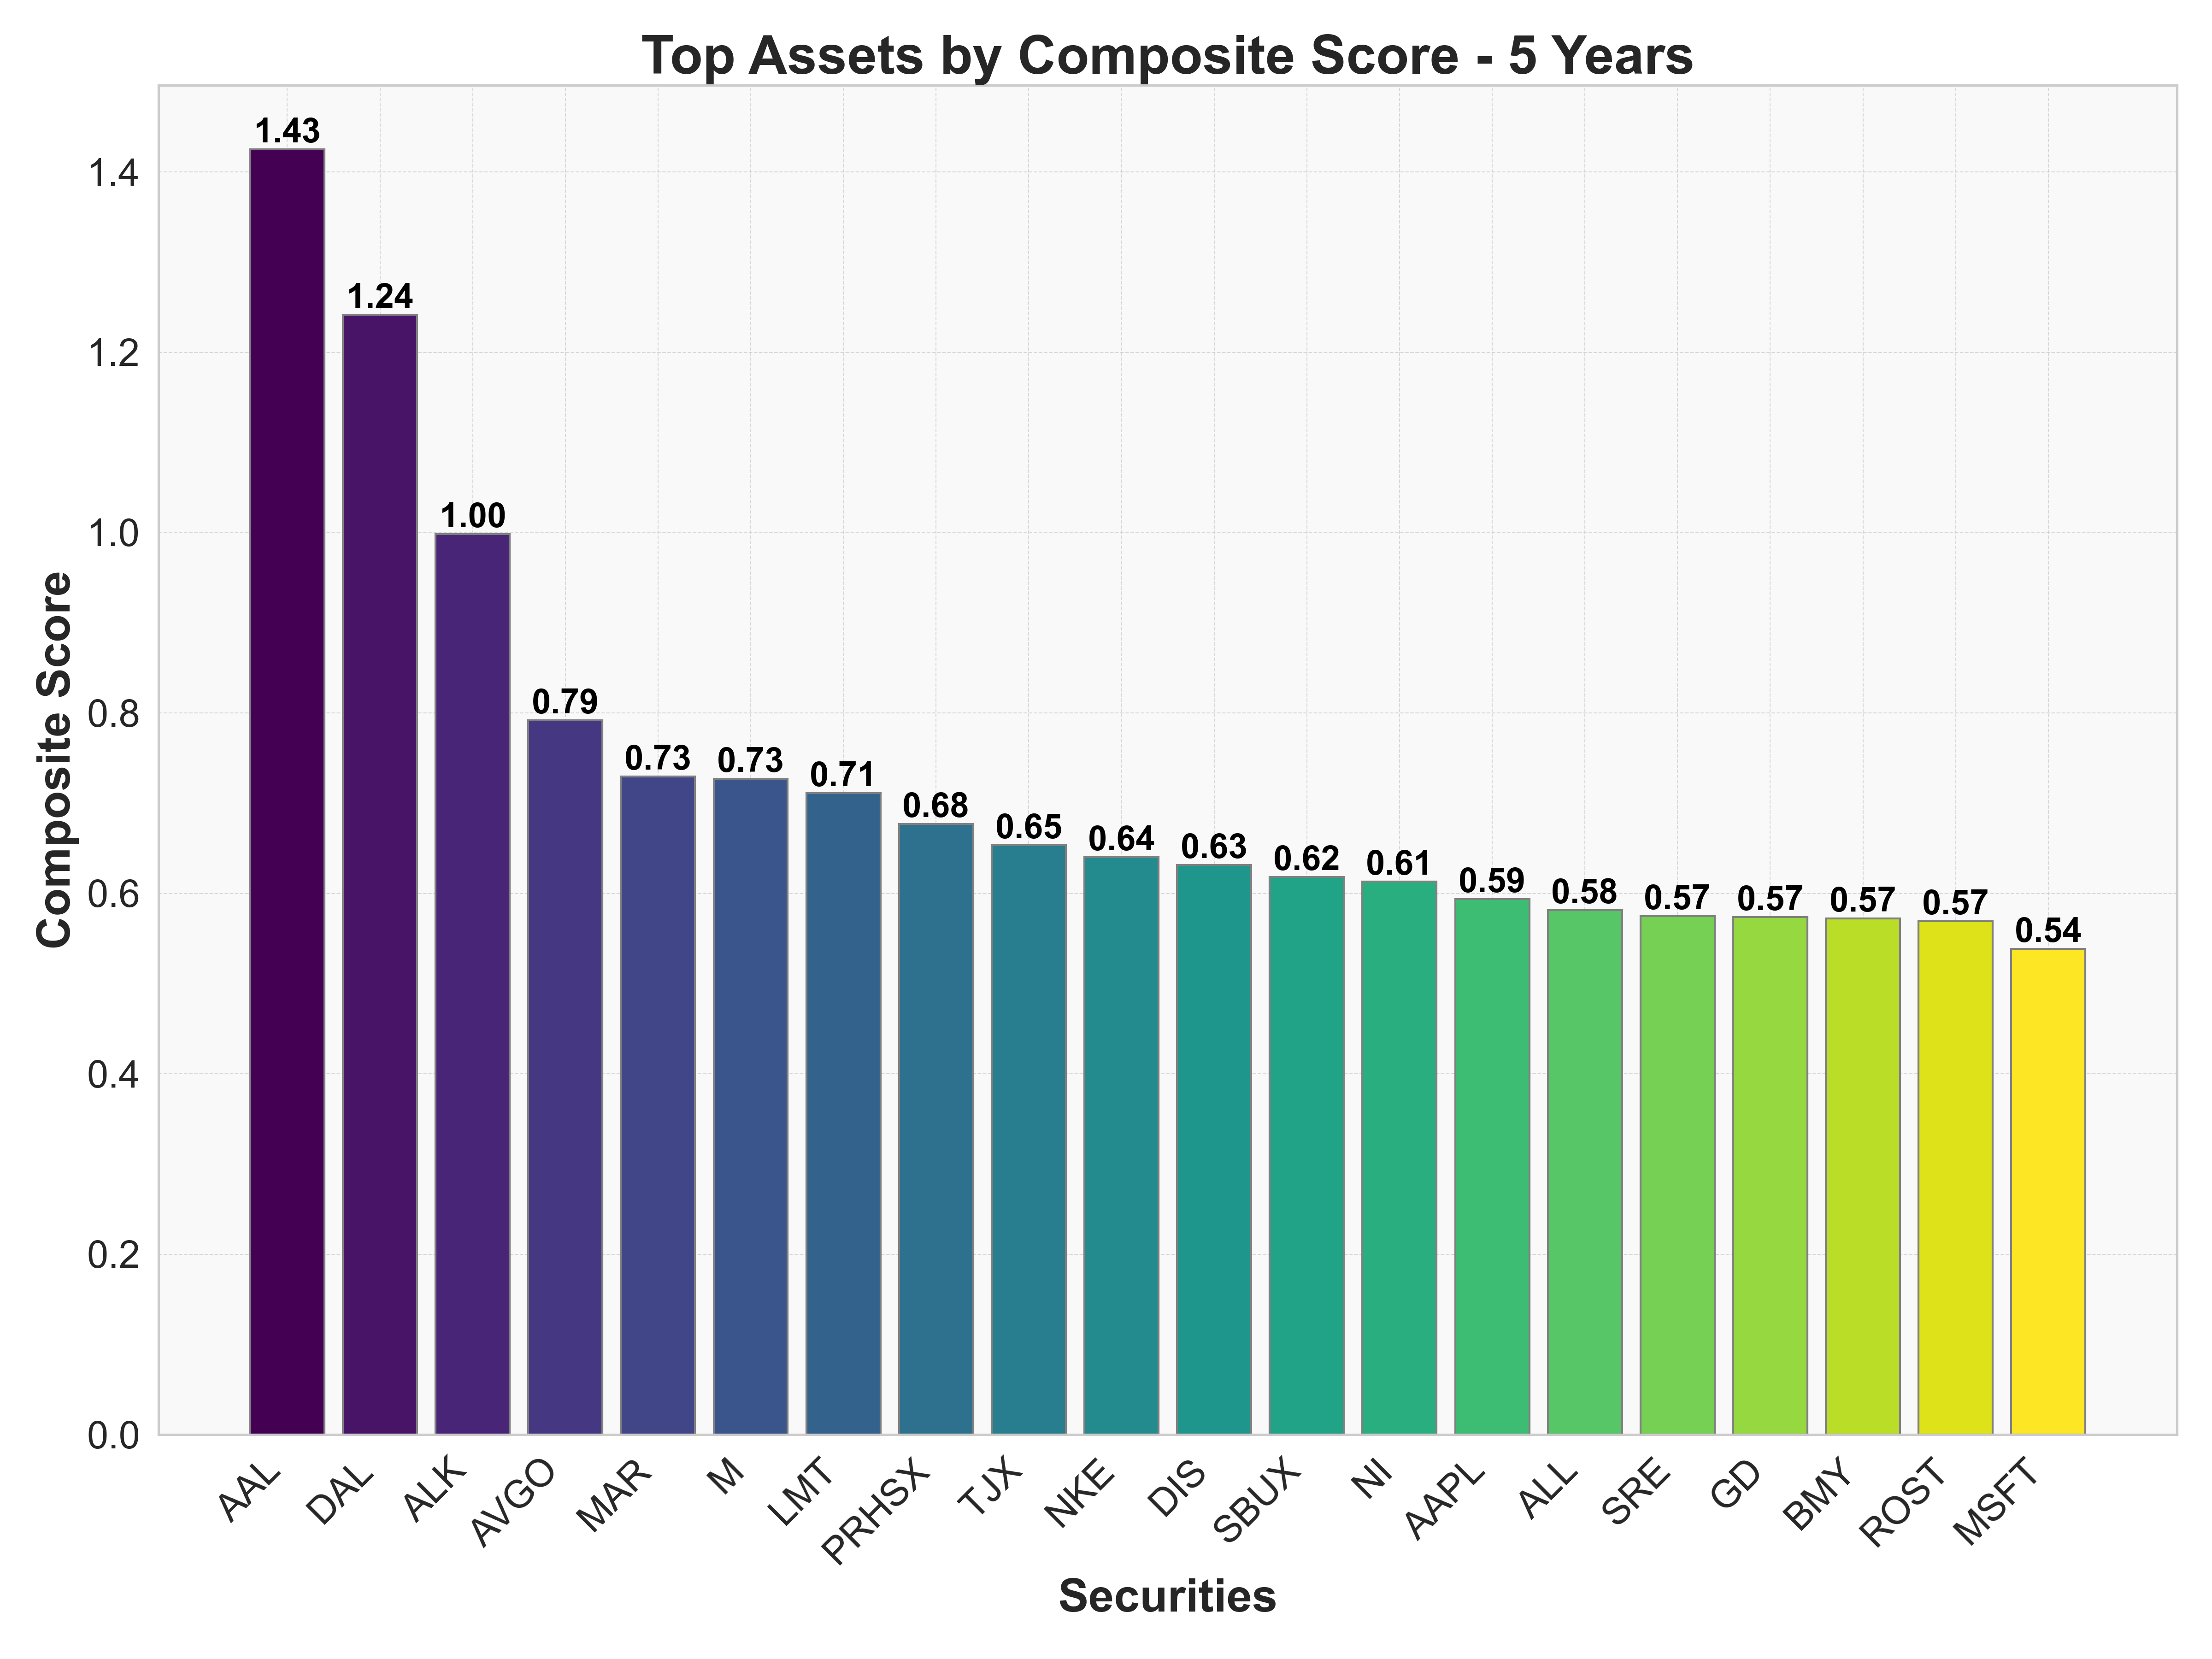
\includegraphics[width=0.8\textwidth]{../Figures/top_assets_composite_score_5_years.png}
    \caption{Top Assets by Composite Score (5 Years)}
    \label{fig:top_assets_5y}
\end{figure}


\newpage

\subsubsection{Optimal Portfolios Composition}


\begin{figure}[!htbp]
    \centering
    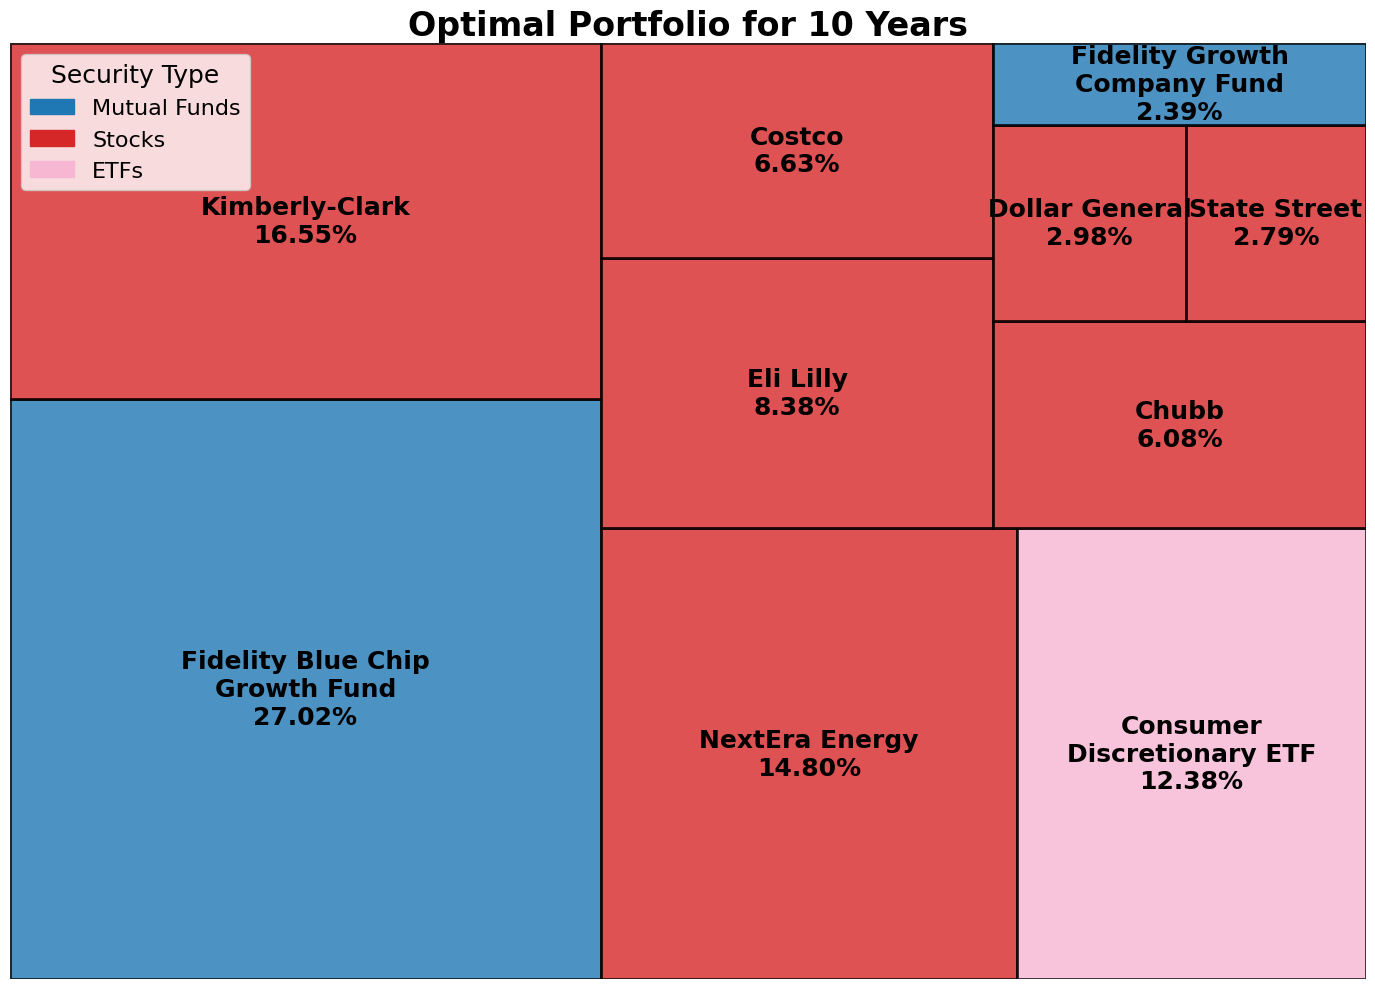
\includegraphics[width=0.8\textwidth]{../Figures/optimal_portfolio_10_years.png}
    \caption{Optimal Portfolio for 10 Years}
    \label{fig:optimal_portfolio_10y}
\end{figure}

\begin{figure}[!htbp]
    \centering
    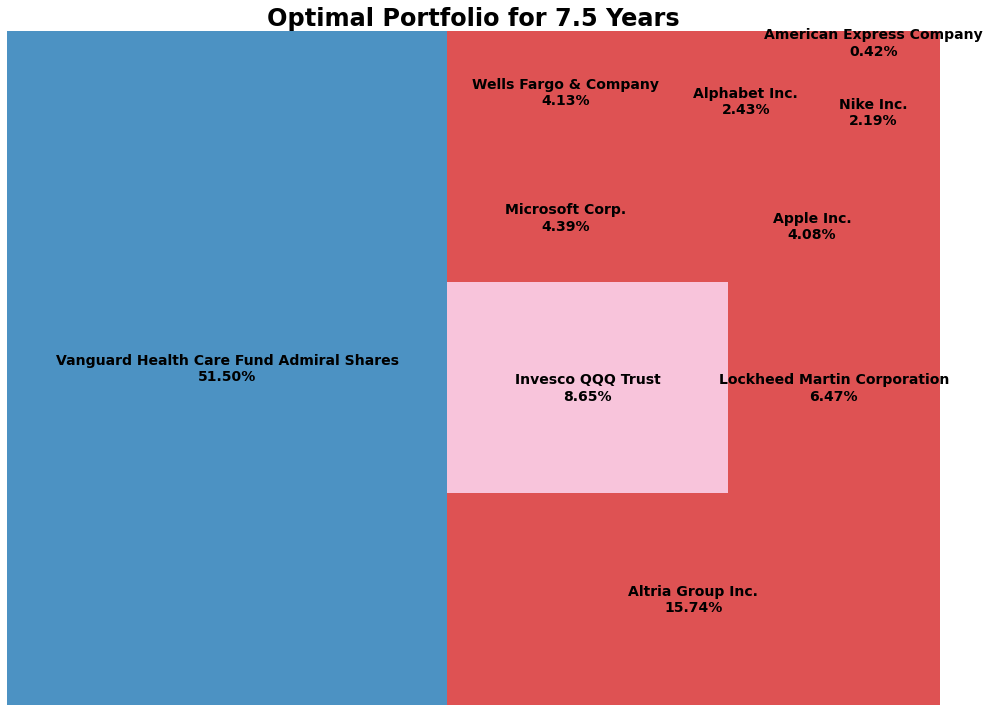
\includegraphics[width=0.8\textwidth]{../Figures/optimal_portfolio_7_5_years.png}
    \caption{Optimal Portfolio for 7.5 Years}
    \label{fig:optimal_portfolio_7_5y}
\end{figure}

\begin{figure}[!htbp]
    \centering
    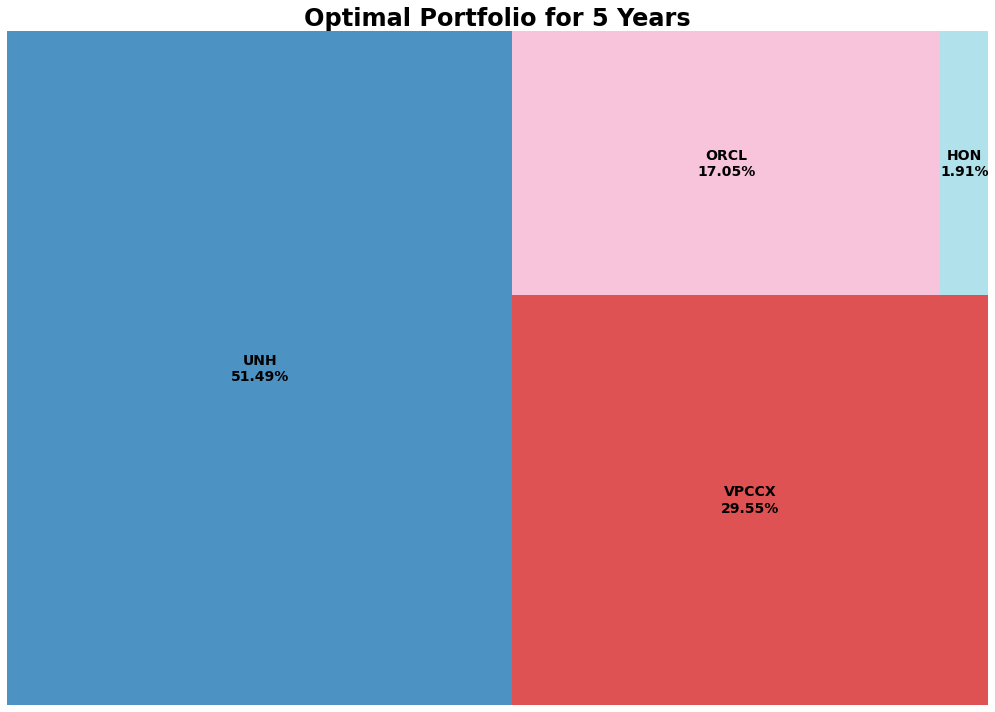
\includegraphics[width=0.8\textwidth]{../Figures/optimal_portfolio_5_years.png}
    \caption{Optimal Portfolio for 5 Years}
    \label{fig:optimal_portfolio_5y}
\end{figure}


\newpage

\subsection{Comparison with Hindsight Data}


\begin{figure}[!htbp]
    \centering
    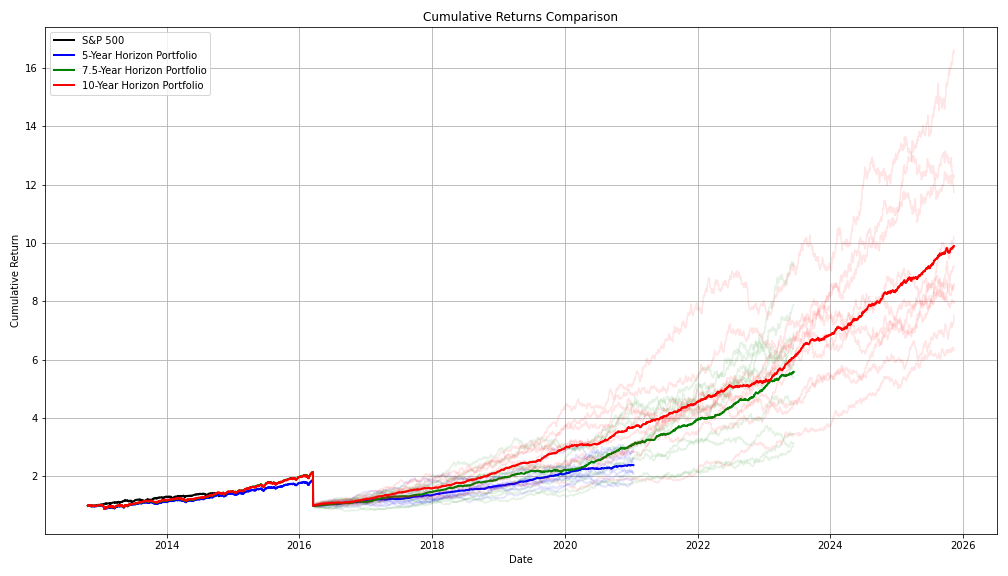
\includegraphics[width=0.8\textwidth]{../Figures/cumulative_returns_comparison.png}
    \caption{Cumulative Returns Comparison of Actual Portfolios vs. S\&P 500}
    \label{fig:cumulative_returns_comparison}
\end{figure}

\subsubsection{Cumulative Returns Summary}

\begin{figure}[!htbp]
    \centering
    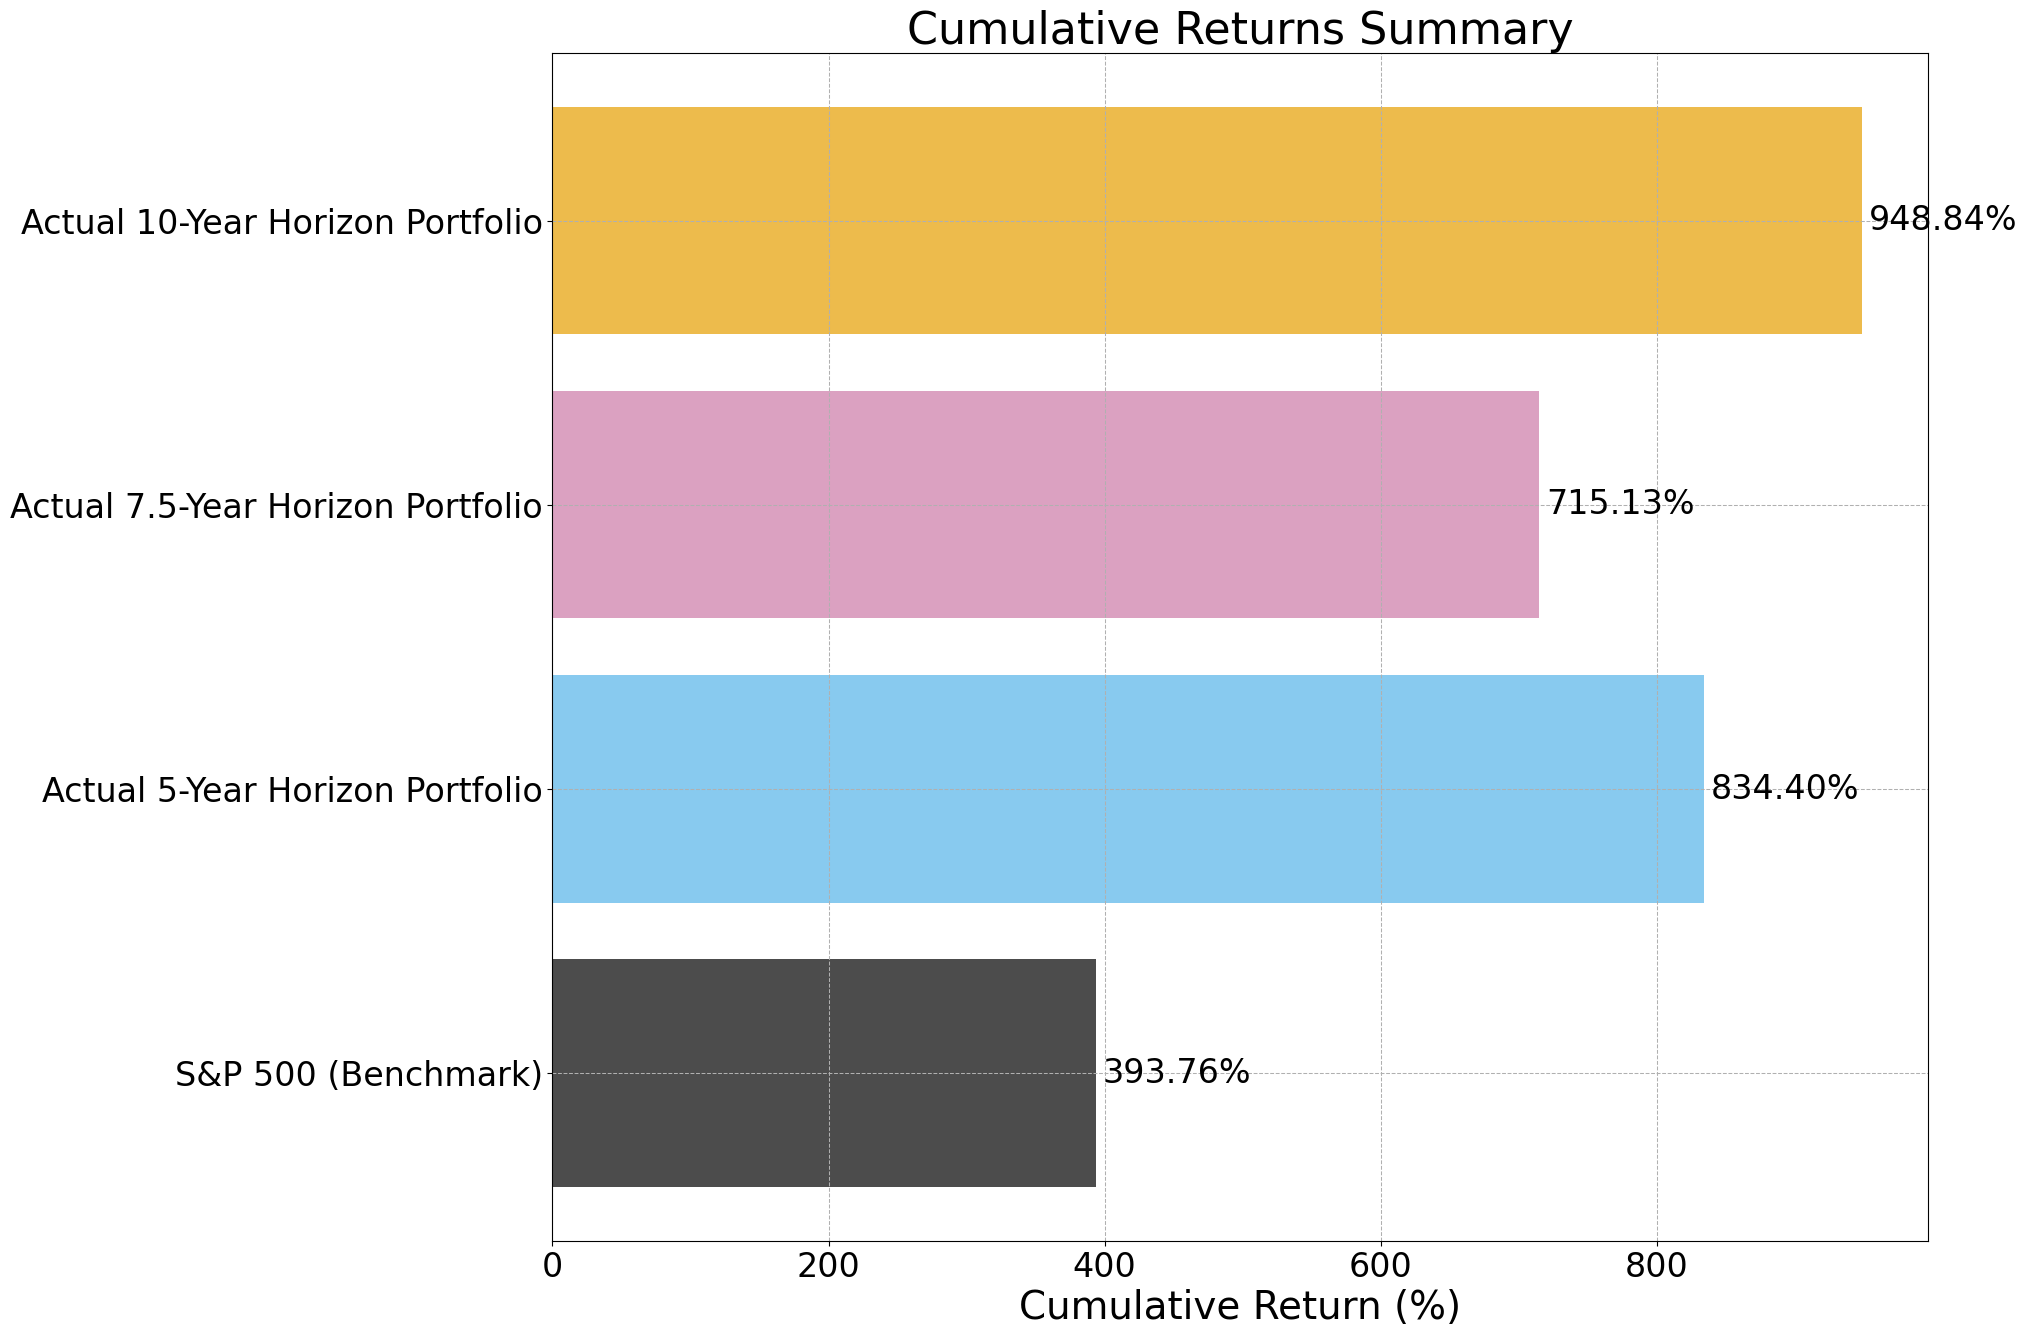
\includegraphics[width=0.8\textwidth]{../Figures/cumulative_returns_summary.png}
    \caption{Cumulative Returns Summary from 2011-05-04 to 2024-07-10}
    \label{fig:cumulative_returns_summary}
\end{figure}




\newpage


\subsection{Monte Carlo Simulation for Future Forecasting}


\begin{figure}[!htbp]
    \centering
    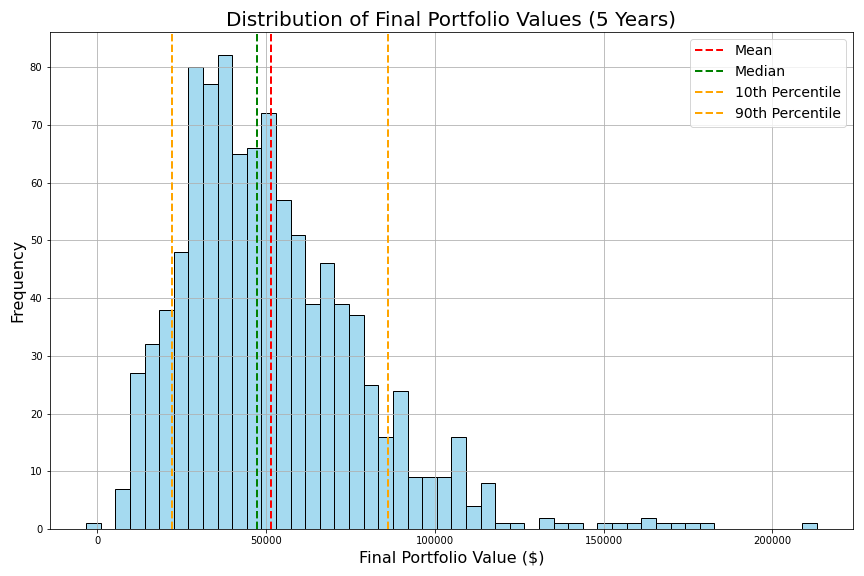
\includegraphics[width=0.8\textwidth]{../Figures/final_portfolio_values_distribution_5_years.png}
    \caption{Distribution of Final Portfolio Values (5 Years)}
    \label{fig:final_portfolio_values_5y}
\end{figure}

\begin{figure}[!htbp]
    \centering
    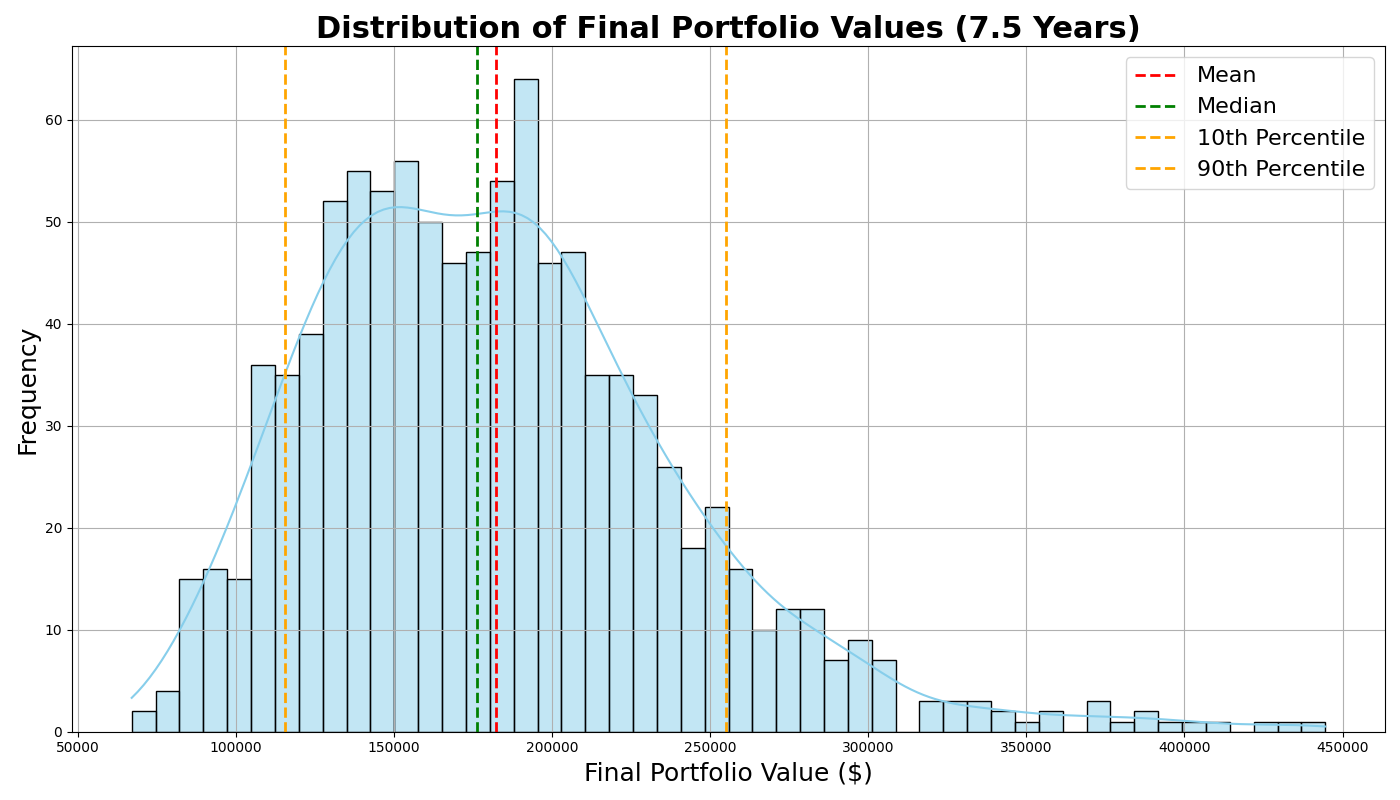
\includegraphics[width=0.8\textwidth]{../Figures/final_portfolio_values_distribution_7_5_years.png}
    \caption{Distribution of Final Portfolio Values (7.5 Years)}
    \label{fig:final_portfolio_values_7_5y}
\end{figure}

\begin{figure}[!htbp]
    \centering
    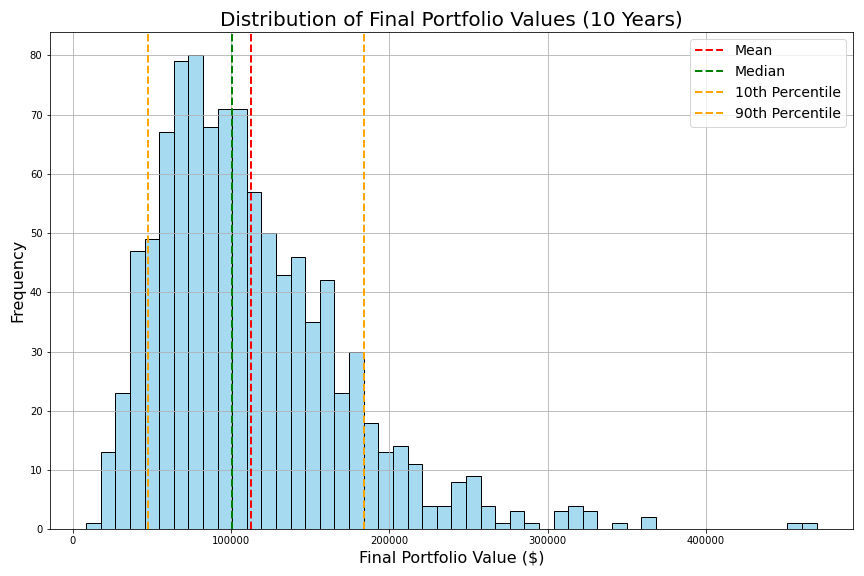
\includegraphics[width=0.8\textwidth]{../Figures/final_portfolio_values_distribution_10_years.png}
    \caption{Distribution of Final Portfolio Values (10 Years)}
    \label{fig:final_portfolio_values_10y}
\end{figure}

\subsubsection{Cumulative Returns Over Time}

\begin{figure}[!htbp]
    \centering
    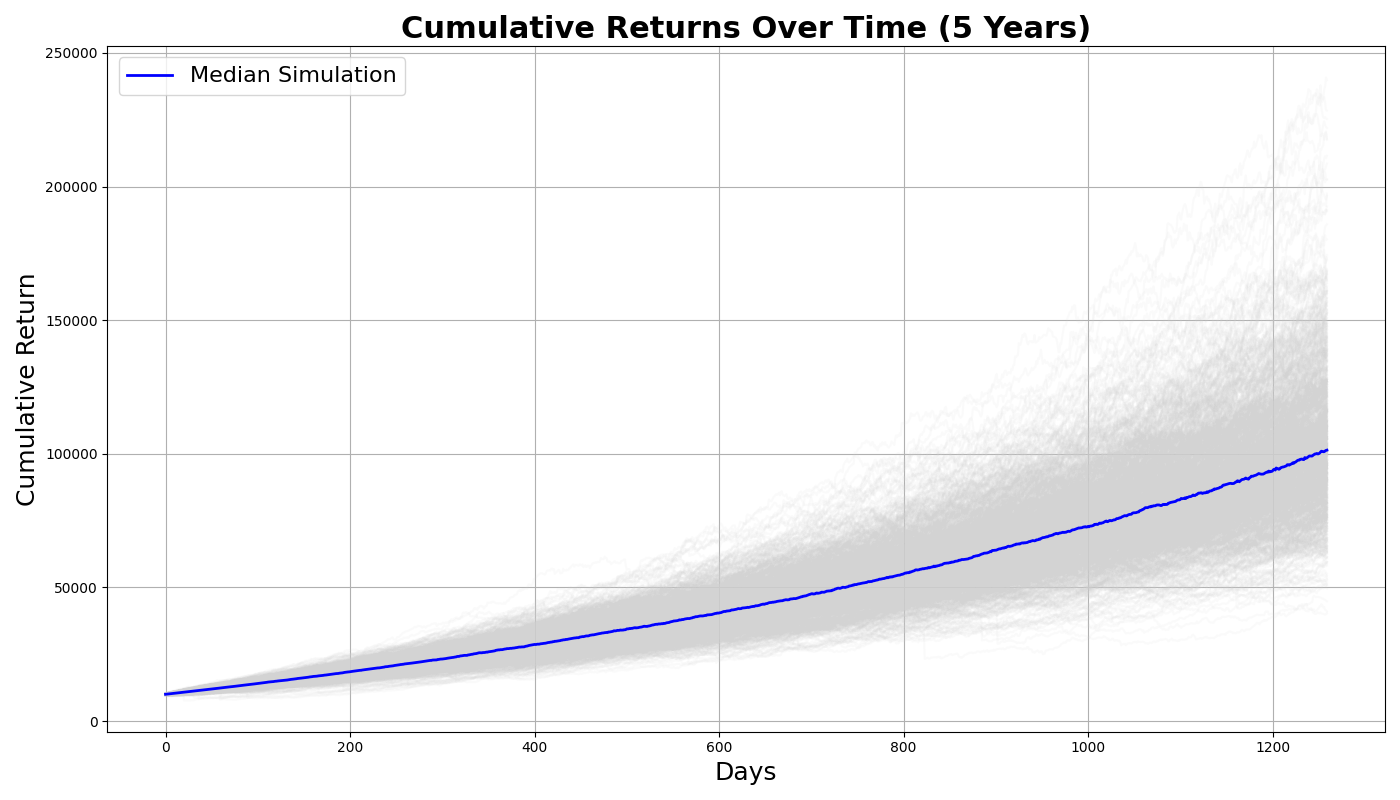
\includegraphics[width=0.8\textwidth]{../Figures/cumulative_returns_over_time_5_years.png}
    \caption{Cumulative Returns Over Time (5 Years)}
    \label{fig:cumulative_returns_5y}
\end{figure}

\begin{figure}[!htbp]
    \centering
    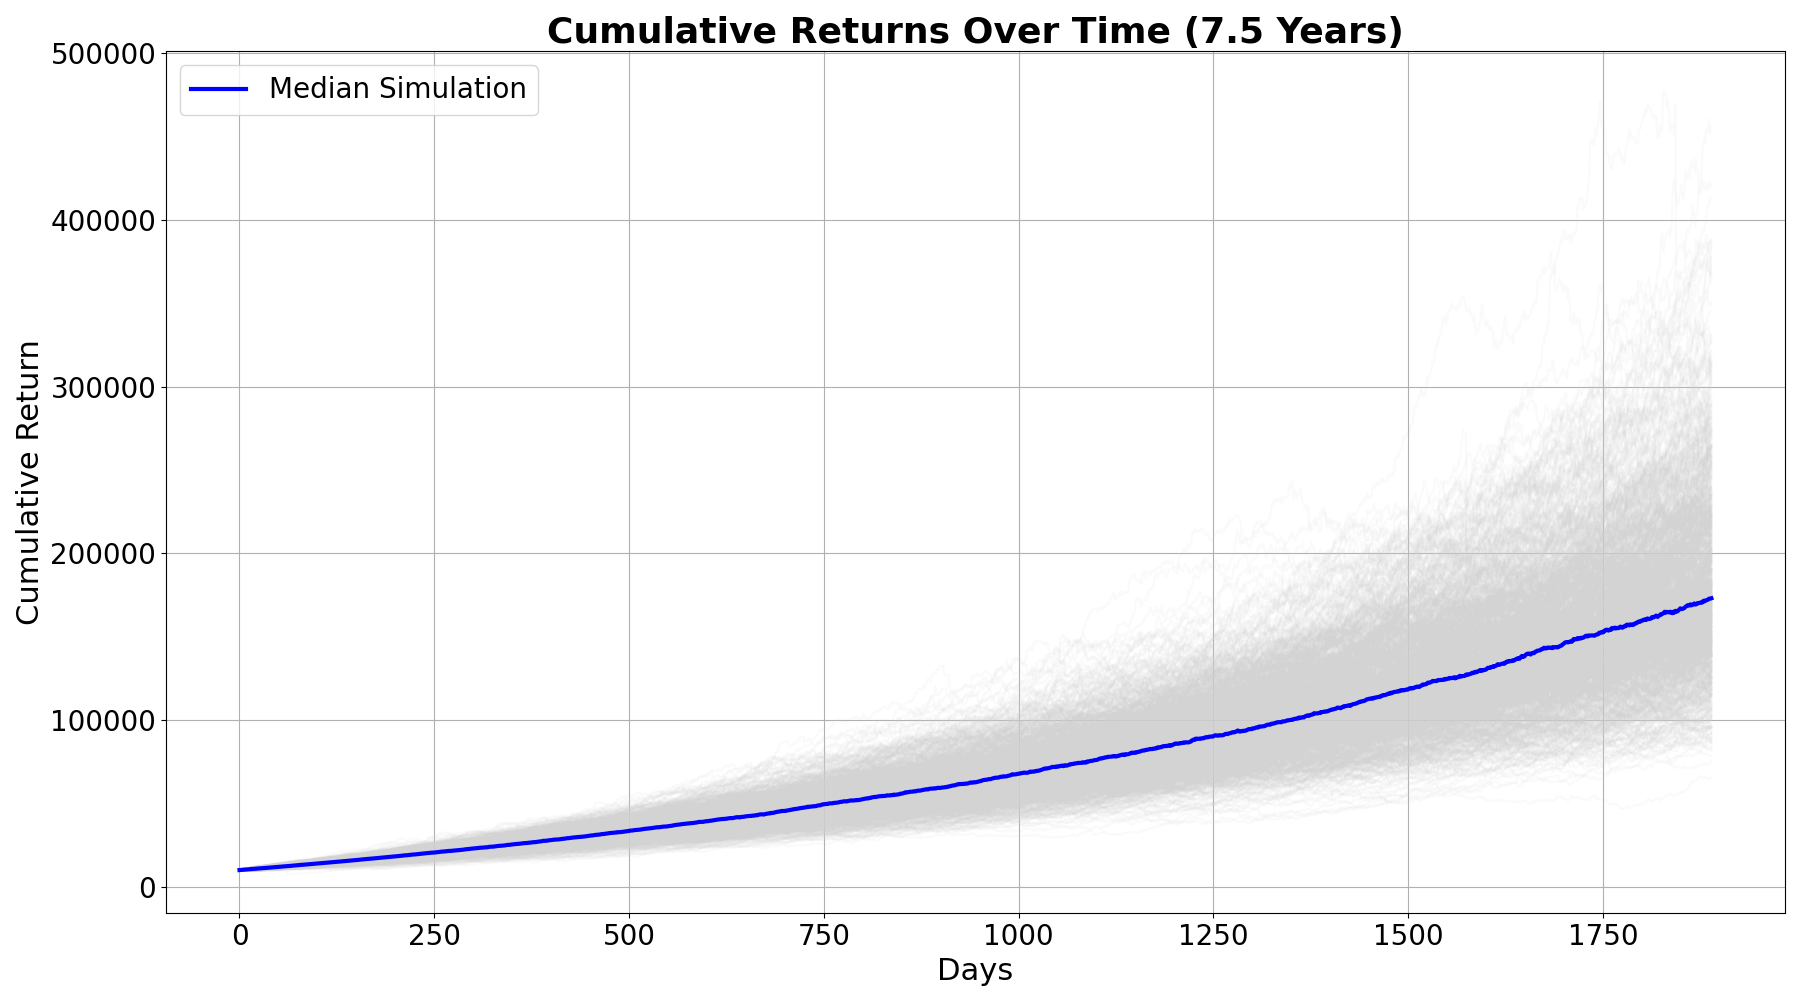
\includegraphics[width=0.8\textwidth]{../Figures/cumulative_returns_over_time_7_5_years.png}
    \caption{Cumulative Returns Over Time (7.5 Years)}
    \label{fig:cumulative_returns_7_5y}
\end{figure}

\begin{figure}[!htbp]
    \centering
    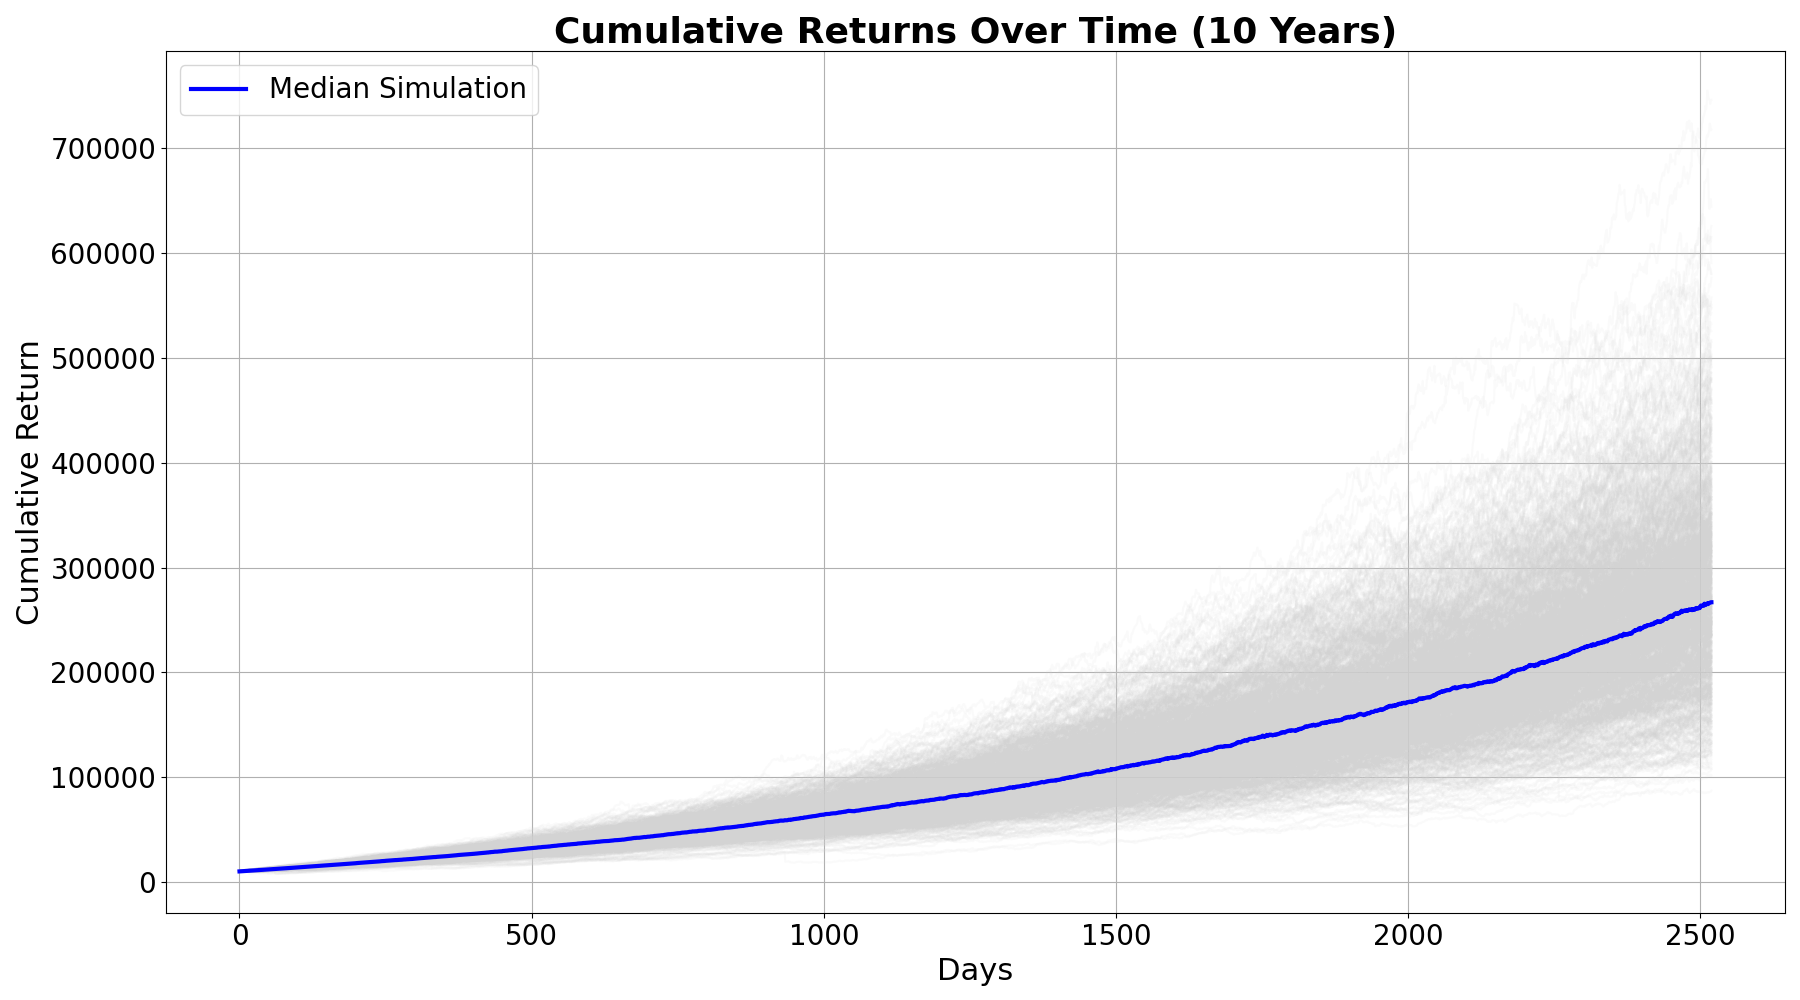
\includegraphics[width=0.8\textwidth]{../Figures/cumulative_returns_over_time_10_years.png}
    \caption{Cumulative Returns Over Time (10 Years)}
    \label{fig:cumulative_returns_10y}
\end{figure}




\subsection{Monte Carlo Forecast Summary}

\begin{table}[h!]
\centering
\scriptsize
\begin{tabular}{lccccccc}
\hline
Statistic & \begin{tabular}[c]{@{}c@{}}Mean Final \\ Portfolio Value (\$)\end{tabular} & \begin{tabular}[c]{@{}c@{}}Median Final \\ Portfolio Value (\$)\end{tabular} & \begin{tabular}[c]{@{}c@{}}10th Percentile Final \\ Portfolio Value (\$)\end{tabular} & \begin{tabular}[c]{@{}c@{}}90th Percentile Final \\ Portfolio Value (\$)\end{tabular} & \begin{tabular}[c]{@{}c@{}}Total Percentage \\ Yield (\%)\end{tabular} & \begin{tabular}[c]{@{}c@{}}Annual Percentage \\ Yield (\%)\end{tabular} \\
\hline
10-Year Horizon & 283094.44 & 265864.65 & 171232.59 & 420935.51 & 2730.94 & 39.70 \\
7.5-Year Horizon & 180745.35 & 173433.88 & 116972.91 & 256760.32 & 1707.45 & 47.10 \\
5-Year Horizon & 101559.42 & 98327.18 & 67062.20 & 139233.79 & 915.59 & 58.98 \\
\hline
\end{tabular}
\end{table}

\textbf Provides a detailed summary of the statistical outcomes for each investment horizon. The mean and median final portfolio values give insights into the expected performance, while the 10th and 90th percentile values offer a perspective on the range of potential outcomes. The total and annual percentage yields reflect the overall return potential of the portfolios over their respective horizons.

\newpage
